\documentclass[]{article}

\usepackage{amsmath,amssymb,amsfonts,amsthm}    % Typical maths resource packages
\usepackage{graphicx}                           % Packages to allow inclusion of graphics
\usepackage{hyperref}   % For creating hyperlinks in cross references
\usepackage[authoryear]{natbib}                 % literature reference style
\usepackage[bf]{caption}
\usepackage{float}
\usepackage{subfig}






% -------------------------------
% --- some layout definitions ---
% -------------------------------

% define topline
\usepackage[automark]{scrpage2}
\pagestyle{scrheadings}
\automark{section}
\clearscrheadings
\ohead{\headmark}

% define citation style
\bibliographystyle{ecta}

% define page size, margin size
\setlength{\headheight}{1.1\baselineskip}
\voffset=-2cm
\hoffset=-3cm
\textheight24cm
\textwidth15.5cm
\topmargin1cm
\oddsidemargin3cm
\evensidemargin3cm

% define line line spacing = 1.5
\renewcommand{\baselinestretch}{1.5}

% define second level for `itemizing'
\renewcommand{\labelitemii}{-}




% --------------------------------------
% --------------------------------------
% --------------------------------------
% --- the structure the tex document ---
% ---  (this our recommendation) -------
% frontmatter:
%   - titlepage (mandatory),
%   - acknowledgement,
%   - abstract,
%   - table of contents (mandatory),
%   - list of abbreviations (not mandatory),
%   - list of figures (not mandatory),
%   - list of tables  (not mandatory) .
%
% body of the thesis (the structure of the thesis body is not mandatory, but the list of literature is mandatory):
%   - introduction,
%   - methods,
%   - data,
%   - results,
%   - conclusion,
%   - literature (mandatory),
%   - appendix (figures, tables).
%
% last page:
%   - declaration of authorship (mandatory).
% --------------------------------------
% --------------------------------------
% --------------------------------------

\begin{document}

% -------------------------------
% --- frontmatter: Title page ---
% -------------------------------

\thispagestyle{empty}




\begin{center}

    {\Large{\bf BIG FIVE PERSONALITIES}} \vspace{0.5cm}


    {\normalsize Project submitted \\\vspace{0.5cm}
    to}\\\vspace{0.5cm}
    {\normalsize{\bf Prof. Dr. Petra Burdejova}} \\\vspace{0.5cm}
    {\normalsize{\bf Prof. Dr. Awdesch Melzer}} \\\vspace{0.5cm}
    {\normalsize Humboldt-Universit\"at zu Berlin \\
    School of Business and Economics \\
   Ladislaus von Bortkiewicz Chair of Statistics}\\


    {\normalsize by \\\vspace{0.5cm}
     Sahnoune Ammar
    (591358)} \vspace{1cm}


    {\normalsize in partial fulfillment of the requirements \\
    for the degree of \\
    {\bf Master of Statistic} \\
    Berlin, August 11, 2018}

\end{center}




% -----------------------------
% --- frontmatter: Abstract ---
% -----------------------------
\newpage
\pagestyle{plain}
\pagenumbering{roman}   % define page number in roman style
\setcounter{page}{1}    % start page numbering
\input{abstract}



% -----------------------------
% --- frontmatter: Contents ---
% -----------------------------
\newpage
\tableofcontents
\clearpage



% -------------------------------
% --- main body of the thesis ---
% -------------------------------
\newpage
\pagestyle{plain}
\setcounter{page}{1}    % start page numbering anew
\pagenumbering{arabic}  % page numbers in arabic style


\section{Introduction}

The Big Five Personality Traits model can help to address these issues. It's a test that can be used to measure a person's most important personality characteristics, and help him to understand which roles suit him best. Recruiters can also use it to find people who have the personality, as well as the skills, to fit the roles that they are hiring for.

Five-dimension personality model presented by Goldberg
is termed as big five model in personality research
(Goldberg, 1992; Sucier and Goldberg, 1998).

The big five personality dimensions include firstly, opennessess
to experience which is the inclination to be imaginative,
independent, and interested in variety. Secondly,
Conscientiousness is the affinity to be prepared, chary,
and disciplined. Thirdly, the propensity to be gregarious,
fun-loving, and warm is known as extraversion. Fourthly,
the tendency to be sympathetic, trusting, and supportive
is termed as Agreeableness. Lastly, neuroticism is the
tendency to be anxious, emotionally destable, and selfblaming (Goldberg, 1993). Research suggests that there is a significant relationship between personality type and career choices but in practice wrong career choice are made due to the ignorance of specific personality type of the individuals
When working with a large data set, it can be useful to represent the entire data set with Numerical methods. Our project consists to find out what could be the reason for someone to have a certain behavior  at the work place. So we worked on the big five personalities :  Introverted/Extroverted,  Neuro , Agreer, Opened  and Conscious .


Many people, perceive the differences between men and women to be large – so large, in fact, that communication between genders may be difficult. Countless examples from popular culture reinforce this view of extreme differences between the sexes – but is it accurate? Men and women have obviously different biological roles when it comes to propagation of the species, but how much they differ psychologically is a more controversial question, one that requires empirical research to answer adequately. Whether the underlying causes of psychological gender differences are evolutionary or socio-cultural, understanding how men and women differ in the ways in which they think, feel, and behave can shed light on the human condition

i specify my work about gender and we are trying to find evidence of this statement by operating some statistical methods with the Statistical Program " R in data analysis and We went to the Hypothesis women were more opened and conscious  than men at the work place
 
 
 

   

\section{Theory and Design}
how to compare two density distributions in males and females according to the Big Five Personalities

\newpage

\section{Theory and Design}
how to compare two density distributions in males and females according to the Big Five Personalities

\begin{figure}[]
\setlength{\abovecaptionskip}{-4pt}
\begin{center}
\includegraphics{Introversion_Extraversion.png}
  \caption{Introversion Extraversion.png}
  \end{center}


{\normalsize{\bf the interpretation:}} \\\vspace{0.5cm}
the representation show that the graph is not symmetric allowing 
the mean wich equal 0.04  for the females and -0.06  for the males 

The result in this case that females are more Introversion/Extraversion than males
\end{figure}


\begin{figure}[]
\setlength{\abovecaptionskip}{-4pt}
\begin{center}
\includegraphics{Neuro.png}
  \caption{Neuro.png}
  \end{center}

{\normalsize{\bf the interpretation:}} \\\vspace{0.5cm}
the representation show that the graph is not symmetric allowing 
the mean witch equal 0.14 for the females and -0.22 for the males 

The result in this case that females are more Neuro  than males
\end{figure}

\begin{figure}[]
\setlength{\abovecaptionskip}{-4pt}
\begin{center}
\includegraphics{Agree.png}
  \caption{Agree.png}
  \end{center}

{\normalsize{\bf the interpretation:}} \\\vspace{0.5cm}
the representation show that the graph is not symmetric allowing 
the mean witch equal 0,18 for the females and -0.27 for the males

The result in this case that females are more Agree  than males
\end{figure}

\begin{figure}[]
\setlength{\abovecaptionskip}{-4pt}
\begin{center}
  \includegraphics{openess.png} 
  \caption{openess.png}
\end{center}

{\normalsize{\bf the interpretation:}} \\\vspace{0.5cm}
the representation show that the graph is not symmetric allowing 
the mean witch equal 0.036 for the females and -0.054 for the males

The result in this case that females are Openess than males
\end{figure}

\begin{figure}[]
\setlength{\abovecaptionskip}{-4pt}
\begin{center}
\includegraphics{Conscient.png}
  \caption{Conscient.png}
  \end{center}


{\normalsize{\bf the interpretation:}} \\\vspace{0.5cm}
the representation show that the graph is not symmetric allowing 
the mean wich equal -0.092 for the females and 0.14 for the males

The result in this case that males are  more Consient  than females

\end{figure}
\begin{figure}[]
\setlength{\abovecaptionskip}{-4pt}
\begin{center}
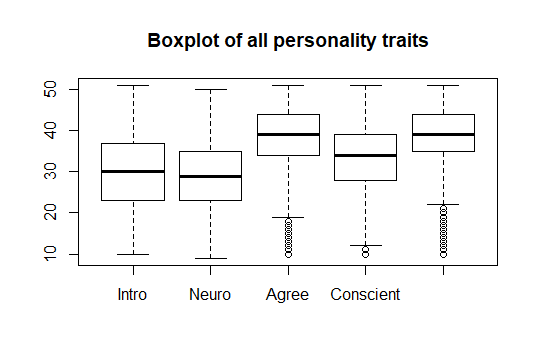
\includegraphics{Boxplot_of_all_personality.png}
  \caption{Boxplot of allpersonality.png}
  \end{center}


{\normalsize{\bf the interpretation:}} \\\vspace{0.5cm}
we observe that the boxplots of introverted/extroverted persons and neuro (isolated) are larger than agreer and opened persons 

\end{figure}







\newpage
\section{Implementation/Simulation}


\underline{Data gender
\href{https://github.com/sahnouna/BIG_FIVE_PERSONALITIES/blob/master/DataAnalysis.R}{\includegraphics[scale = 0.06]{Figures/qletlogo.pdf}} :} 
\newline 
This Quantlet translates data sets containing answers to a 50 item questionnaire into a data frame with the values of the personality traits according to the evaluation key. Optionally it can also deal with a data set from a questionnaire about grit. However, the data needs to contain the 50 items of the personality test. The order in which these answers are given does not matter since they are going to be reordered in the process of data cleaning.
\newline
This file deals with an analysis of all five personality traits (Extraversion, Openness, Conscientiousness, Agreeableness, and Neuroticism) with accordance to the gender(males and females) . In short, we analysis the personality among to compare the mean of males and the mean of females . Note, that the analysis from this file was made for a visual interpretation.
 \newline \newline
 In our study we have tried to show such patterns as well. For that we wanted to receive a visual big picture of the personality traits across the gender with accordance to our data set. 
Our file, in which we applied this study, starts with the general data generation part. With the function source(), we are able to access another file or rather script in order to connect with the already prepared data set which we will need for this study
The data "clean" function 
The data "clean" function mean takes the name of a data set, a boolean variable whether the data contains grit questionnaire and a survey date as parameters. This function can deal with excel data and data in the .csv format. It converts some of the numerical variable into factors and reorders the column. Before columns are converted the function checks whether they are null to prevent errors when trying to convert non existing columns.
\newline
\underline{DataAnalysis
\href{https://github.com/sahnouna/BIG_FIVE_PERSONALITIES/blob/master/DataAnalysis.R}{\includegraphics[scale = 0.06]{Figures/qletlogo.pdf}} :} 
\newline 

This Quantlet have This file deals with an analysis of all five personality traits (Extraversion, Openness, Conscientiousness, Agreeableness, and Neuroticism) with accordance to the gender(males and females) in two diffrents  country(USA and GB) . In short, we analysis the personality among to compare the mean of males and the mean of females . Note, that the analysis from this file was made for a visual interpretation
 In our study we have tried to show such patterns as well. For that we wanted to receive a visual big picture of the personality traits across the gender with accordance to our data set. 
Our file, in which we applied this study, starts with the general data generation part. With the function source(), we are able to access another file or rather script in order to connect with the already prepared data set which we will need for this study
The data "clean" function 
The data "clean" function mean takes the name of a data set, a boolean variable whether the data contains grit questionnaire and a survey date as parameters. This function can deal with excel data and data in the .csv format. It converts some of the numerical variable into factors and reorders the column. Before columns are converted the function checks whether they are null to prevent errors when trying to convert non existing columns.
\newline
\underline{Data Preparation  \href{https://github.com/sahnouna/BIG_FIVE_PERSONALITIES/blob/master/DataPreparation.R}{\includegraphics[scale = 0.06]{Figures/qletlogo.pdf}} :} 

In this Quantlet we test how well principal component analysis and factor analysis estimate the scaled values obtained by using the evaluation key. Throughout this analysis the data worked with will often be just the answers to the questionnaires. To that end the columns will be selected using to numbers. 'Start' which is set to "which(colnames(data) == "E1")" and 'end' which is set to 'start + 49'. This is possible since the columns where sorted in this specific way during data cleaning.
\newline
The first step is estimating the correct number of pcs or factors to extract. This is done in several ways.
The first way is using the function implemented in R, which estimates the number of factors in a factor analysis. Another method is to do a parallel analysis to find both a good number for factors and pcs. The last method implemented is to do a simple PCA and to draw a screeplot. 
\newline
In the code there are 3 functions implemented to extract the values via PCA as well as 1 function that uses factor analysis . Those 4 functions all take a cleaned data frame as input and return a new data frame in which the questionnaire answers are replaced by the estimated values for the personality traits. Non-questionnaire columns remain unchanged. The functions for PCA differ in the PCA function they use.  
\newline
Next the results of 'prcomp' and 'princomp' are compared in 2 ways. First, a screeplot is drawn for both results and then their centers and standard deviations are compared.
\newline
The main comparison of PCA, factor analysis and the evaluation key is done in two functions: 'compareDensities' and 'compareDifferences' . Both function take the name of a data file as input. Then both transform the questionnaire answers to personality traits using the evaluation key, factor analysis and PCA ('princomp'). 'compareDensities' then uses a for loop to go through a vector with the names of the personality traits and draws a a plot containing the density distribution of all 3 methods for each personality trait.
\newline
'compareDifferences' simply compares the average difference between factor analysis and evaluation key vs. PCA and evaluation key.
\newline
In the data cleaning part it was mentioned that there is an option to combine 2 data set in order to have more observations. This is only possible if both data sets don't have overlap. Otherwise you would have the several observations twice in the combined data set. 
\newline
The last part of this analysis is a test to check for overlap between 2 datasets. To do this the 2 data sets are merged by the traits or by the remaining columns. The 'nrow' function then gives the number of matching pairs in the 2 data sets.  


\newpage
\section{Empirical Study/ Testing}



we tested our Data gender.R with P-value and T-student  to see whether it is significant or not  and then we compare  the mean of males and the mean of  females  to see which one of gender have a special personality 

we concluded that in this table :

\begin{table}[ht]
    \begin{center}
        {\footnotesize
        \begin{tabular}{l|l|l|l|l|l|}
        \hline \hline
               & introversion   & neuro    & agree   & openess   & conscient        \\
            \hline
                Mean of males    & -0,06 & -0,22   & -0,27 & -0,054 & 0,14   \\
                Mean of females  & 0,04 & 0,14 & 0,18 & 0,036 & -0,092  \\
                t-student        & 7 & 25 & 31,5 & 6 & 16   \\
                p-value          & 1,213e-12 & 2,2e-16 & 2,2e-16 & 3,373e-10 & 2,2e-16   \\
               
            \hline \hline
        \end{tabular}}
    \end{center}
    
\end{table}

{\normalsize{\bf the results:}} \\\vspace{0.5cm}


we see that the t-student is bigger than T-table wich equal 1,65  with α=0,05     and  Degree of freedom (DF) is bigger than 29
  P-value is smaller than 0,05
and this confirm our rejection hypothesis that mean not equal to zero (or the mean of the females not equal the mean of males) 
  in case Introversion/Extraversion , Neuro, Agree and Openess
we see that the mean of the males is smaller than  the mean of  the females and that mean females are more Introversion/Extraversion,neuro, agree and openness than males
But in case Consient we see that the mean of the males is bigger than  the mean of  the females and that mean males are more consient than females 

















\newpage
\section{Conclusions}\label{Sec:Conc}
The  hypothesis was that Women were opened and more conscious than men at the workplace. The  results of our work  do not  support at all this hypothesis.

We think the tests we ran went  smoothly and we had no problems, except for the fact that we observe a certain difference when working on Consciousness of a worker . Therefore, we had to take the measurements quickly. So we found that our theory was half true and half false (concerning the fact that women were more conscious than men).

An interesting future study might involve testing the effectiveness of the worker at the workplace such that we ask ourselves whether opened women are more effective than conscious men at the workplace





\section{Refernces}

Goldberg LR (1992). The development of markers for Big Five Factor
Struct. Psychol.

Goldberg LR (1993). The Structure of Phenotypic Personality Traits.
Am. Psychol., 
 

 
  





% ----------------
% --- appendix ---
% ----------------
\appendix

% literature
\newpage
\addcontentsline{toc}{section}{References}
\bibliography{literature}

% figures (not mandatory)
\newpage
\input{app_figures}

% tables (not mandatory)
\newpage
\input{app_tables}



% --------------------------------------------
% --- last page: Declaration of Authorship ---
% --------------------------------------------

\newpage
\thispagestyle{empty}
%{\Large{\bf Declaration of Authorship}}\vspace{0.5cm}

\section*{Declaration of Authorship}

We hereby confirm that we have authored this Seminar paper independently and without use
of others than the indicated sources. All passages which are literally or in general matter taken
out of publications or other sources are marked as such.
\vspace{1cm}

Berlin, August 12, 2018 \vspace{0.5cm}

Ammar Sahnoune 

(591358)



\end{document}
